% Copyright 2026 Sreeram Anil
% SPDX-License-Identifier: CC-BY-4.0
% =============================================================================
%  Student's t filter — robust_kalman family
% =============================================================================
\providecommand{\vf}{\bm{f}} \providecommand{\vh}{\bm{h}}
\providecommand{\vd}{\bm{d}} \providecommand{\mM}{\bm{M}}
\providecommand{\va}{\bm{a}} \providecommand{\vb}{\bm{b}}

\chapter{Student's t filter (StudentT-KF)}
\label{ch:studenttkf}

\section*{At a glance}
\begin{tabular}{@{}l>{\raggedright\arraybackslash}p{0.76\textwidth}@{}}
Family & Robust / embedded Kalman \\
Header & \texttt{include/estkit/filters/student\_t\_kf.hpp} \\
Registered name & \texttt{StudentT-KF} \\
State dimension & $n_x = 4$ (cell model) --- generic in $n_x, n_u, n_y$ \\
Cost per step & $\mathcal{O}(N_{\mathrm{fp}} n_x^2 n_y + n_x^3)$; 696\,ns/step, 4568\,B, no heap \\
Primary references & \cite{roth2013studentt,agamennoni2012heavytailed,huang2016robustt,kotz2004multivariatet} \\
\end{tabular}

\section{Motivation and aerospace/BMS relevance}
The Huber and correntropy filters of the preceding chapters are \emph{estimators}: they replace a
quadratic loss by a robust one and are justified by a minimax-variance or a similarity argument.
The Student's t filter is a \emph{model}: it says that the noise is genuinely heavy-tailed, writes
down a probability density that says so, and derives the Bayesian update.  Everything --- the
weight function, the covariance inflation, the recovery after an outlier --- then follows from the
model rather than from a tuning choice, and the single parameter $\nu$ (degrees of freedom) has a
clear meaning: $\nu\to\infty$ is Gaussian, $\nu=3$ has infinite kurtosis, $\nu\le2$ has infinite
variance.

This matters for a BMS because the voltage measurement chain really is heavy-tailed rather than
merely occasionally wrong.  Between the ordinary ADC noise and the gross faults there is a
continuum: switching transients that add a few millivolts, sampling jitter during a fast current
ramp, a slightly noisy sense lead.  A contamination model ($1-\varepsilon$ Gaussian plus
$\varepsilon$ garbage) describes the two ends; a $t$ distribution describes the whole range with
one parameter.

The chapter also reports a negative result that is worth as much as the positive one.  Roth,
{\"O}zkan \& Gustafsson's closed-form recursion \cite{roth2013studentt} --- the exact conditional
of a multivariate $t$ plus moment matching of the degrees of freedom --- is derived in full in
\S\ref{sec:st-exact}, and it is then shown, analytically and experimentally, that it cannot be run
recursively on this problem: its multiplicative scale update has a negative logarithmic drift and
the filter collapses within a few hundred samples.  The implemented filter therefore uses the
independent-scale (variational) form of the same $t$ model, \S\ref{sec:st-vb}, which is
unconditionally stable and keeps the whole $t$ apparatus.

\section{Problem statement and assumptions}
\begin{definition}[Multivariate Student's t]\label{def:st-t}
$\vx\sim\mathrm{St}(\bm\mu,\bm\Sigma,\nu)$ with location $\bm\mu\in\real^{n}$, \emph{scale matrix}
$\bm\Sigma\succ0$ and $\nu>0$ degrees of freedom has density
\begin{equation}
p(\vx)\propto
\Big[1+\tfrac1\nu(\vx-\bm\mu)^\T\bm\Sigma^{-1}(\vx-\bm\mu)\Big]^{-\frac{\nu+n}{2}},
\label{eq:st-pdf}
\end{equation}
mean $\bm\mu$ ($\nu>1$) and covariance
\begin{equation}
\Var{\vx}=\frac{\nu}{\nu-2}\,\bm\Sigma \qquad (\nu>2).
\label{eq:st-cov}
\end{equation}
Equivalently, $\vx\,|\,u\sim\N{\bm\mu}{\bm\Sigma/u}$ with $u\sim\mathrm{Gamma}(\nu/2,\nu/2)$: a
$t$ is a Gaussian \emph{scale mixture}, and $u$ is the latent scale.
\end{definition}

\begin{remark}[Scale is not covariance]\label{rem:st-scale}
\eqref{eq:st-cov} is a constant source of errors.  \code{Model::Q} and \code{Model::R} in
\code{estkit} are \emph{covariances}; the filter converts them with
$\bm\Sigma=\frac{\nu-2}{\nu}\,\mathrm{Cov}$ on input (\code{opts.cov\_to\_scale}) and converts back
for the reported \code{P()}.  Skipping this makes the filter assume $\nu/(\nu-2)$ times the
intended noise level --- a factor of $3$ at $\nu=3$.
\end{remark}

The model is
\begin{align}
\vx_{k+1}&=\vf(\vx_k,\vu_k)+\vw_k, & \vw_k&\sim\mathrm{St}(\bm 0,\bm\Sigma_{Q,k},\nu_w),
  \label{eq:st-f}\\
\vy_k&=\vh(\vx_k,\vu_k)+\vv_k, & \vv_k&\sim\mathrm{St}(\bm 0,\bm\Sigma_{R,k},\nu_v),
  \label{eq:st-h}\\
\vx_0&\sim\mathrm{St}(\xhat_0,\bm\Sigma_0,\nu_0). & &
  \label{eq:st-x0}
\end{align}

\section{Derivation}

\subsection{Exact conditional and the closed-form recursion}\label{sec:st-exact}
\begin{lemma}[Conditional of a multivariate t]\label{lem:st-cond}
If $\begin{bmatrix}\vx\\\vy\end{bmatrix}\sim
\mathrm{St}\!\left(\begin{bmatrix}\bm\mu_x\\\bm\mu_y\end{bmatrix},
\begin{bmatrix}\bm\Sigma_{xx}&\bm\Sigma_{xy}\\\bm\Sigma_{yx}&\bm\Sigma_{yy}\end{bmatrix},\nu\right)$
then
\begin{equation}
\vx\,|\,\vy \sim \mathrm{St}\Big(
\bm\mu_x+\bm\Sigma_{xy}\bm\Sigma_{yy}^{-1}(\vy-\bm\mu_y),\;
\frac{\nu+\Delta^2}{\nu+n_y}\big(\bm\Sigma_{xx}-\bm\Sigma_{xy}\bm\Sigma_{yy}^{-1}\bm\Sigma_{yx}\big),
\;\nu+n_y\Big),
\label{eq:st-cond}
\end{equation}
with $\Delta^2=(\vy-\bm\mu_y)^\T\bm\Sigma_{yy}^{-1}(\vy-\bm\mu_y)$
\cite[Ch.~1]{kotz2004multivariatet}.
\end{lemma}

If the predicted state and the measurement noise share the \emph{same} latent scale $u$ and the
same $\nu$, then $[\vx;\vy]$ is jointly $t$ with
$\bm\Sigma_{xy}=\Pminus\mH^\T$ and $\bm\Sigma_{yy}=\mS=\mH\Pminus\mH^\T+\bm\Sigma_R$, and
Lemma~\ref{lem:st-cond} gives the closed-form measurement update
\begin{align}
\mS_k&=\mH_k\Pminus_k\mH_k^\T+\bm\Sigma_{R,k}, \qquad
\veps_k=\vy_k-\vh(\xminus_k,\vu_k), \label{eq:st-S}\\
\Delta_k^2&=\veps_k^\T\mS_k^{-1}\veps_k, \qquad
\mK_k=\Pminus_k\mH_k^\T\mS_k^{-1}, \label{eq:st-D}\\
\xplus_k&=\xminus_k+\mK_k\veps_k, \label{eq:st-x}\\
\Pplus_k&=\frac{\nu+\Delta_k^2}{\nu+n_y}\big(\Pminus_k-\mK_k\mS_k\mK_k^\T\big),\qquad
\nu^+=\nu+n_y. \label{eq:st-P}
\end{align}

The time update is not closed: $\mF\vx+\vw$ is a sum of two independent $t$ vectors, which is not
$t$.  Roth et al.\ approximate it by a $t$ with $\nu^\star=\min(\nu_1,\nu_2)$ --- the heavier tail
--- after rescaling both scale matrices so that the \emph{covariances} are preserved:
\begin{equation}
\bm\Sigma\big|_{\nu^\star}=\bm\Sigma\big|_{\nu_1}\cdot
 \frac{\nu_1(\nu^\star-2)}{\nu^\star(\nu_1-2)},
\qquad
\Pminus_{k+1}=\mF_k\tilde{\bm\Sigma}\mF_k^\T+\tilde{\bm\Sigma}_Q,
\qquad \nu\leftarrow\nu^\star.
\label{eq:st-mm}
\end{equation}
The same rescaling is applied before \eqref{eq:st-S} so that the state and the measurement noise
share one $\nu$.  With $\nu_w=\nu_v+n_y$ the degrees of freedom settle into the two-step cycle
$\nu^-=\nu_v$, $\nu^+=\nu_v+n_y$.

\subsection{Why the closed form cannot be iterated here}\label{sec:st-fail}
Two properties of \eqref{eq:st-S}--\eqref{eq:st-mm} make it unusable on a long, weakly informative
record.

\begin{remark}[No outlier rejection in the mean]\label{rem:st-nomean}
\eqref{eq:st-x} with \eqref{eq:st-D} is \emph{exactly} the Kalman mean.  This is not an accident:
with one shared latent scale $u$, both $\Pminus$ and $\bm\Sigma_R$ are divided by the same $u$, and
the gain $\mK=\Pminus\mH^\T(\mH\Pminus\mH^\T+\bm\Sigma_R)^{-1}$ is invariant to a common scaling.
The shared-scale $t$ filter therefore reacts to a $50$\,mV spike exactly as the EKF does; its only
robustness is the covariance inflation \eqref{eq:st-P}, which speeds up the \emph{recovery} at the
next sample but does not prevent the jump.
\end{remark}

\begin{proposition}[Geometric collapse of the scale matrix]\label{prop:st-collapse}
Combine \eqref{eq:st-P} and \eqref{eq:st-mm} over one predict/update cycle with
$\nu_w=\nu_v+n_y$ and express the result in covariance units.  Then
\begin{equation}
\mathrm{Cov}^+_k = \mathrm{Cov}^{+,\mathrm{KF}}_k\cdot\lambda_k,
\qquad
\lambda_k=\frac{\nu-2+\delta_k^2}{\nu-1},
\qquad
\delta_k^2=\veps_k^\T\mS_{\mathrm{cov},k}^{-1}\veps_k,
\label{eq:st-lambda}
\end{equation}
where $\mathrm{Cov}^{+,\mathrm{KF}}$ is the Kalman posterior covariance and
$\mS_{\mathrm{cov}}$ the covariance-domain innovation covariance.  Under the nominal hypothesis
$\delta_k^2\sim\chi^2(n_y)$, so $\E{\lambda_k}=1$: the recursion is unbiased in the mean.  But
$\chi^2$ is strongly right-skewed --- for $n_y=1$ its median is $0.455$ --- so
$\E{\log\lambda_k}<0$ and the product $\prod_k\lambda_k$ drifts to zero geometrically.
\end{proposition}
\begin{proof}[Sketch]
Substituting the rescaling factors of \eqref{eq:st-mm} into \eqref{eq:st-P} and using
$\mathrm{Cov}=\frac{\nu}{\nu-2}\bm\Sigma$ twice gives \eqref{eq:st-lambda} directly.
$\E{\delta^2}=1$ gives $\E{\lambda}=1$.  For the logarithm, a second-order expansion about
$\delta^2=1$ yields $\E{\log\lambda}\approx-\Var{\delta^2}/\big(2(\nu-1)^2\big)=-1/(\nu-1)^2<0$;
a numerical quadrature at $\nu=4$, $n_y=1$ gives $\E{\log\lambda}=-0.069$ per step.
\end{proof}

A negative logarithmic drift is harmless only if something restores the scale.  The restoring
mechanism is the feedback through $\delta^2$: a smaller $\mathrm{Cov}$ makes
$\mS_{\mathrm{cov}}=\mH\,\mathrm{Cov}\,\mH^\T+\mR$ smaller and $\delta^2$ larger, which pushes
$\lambda$ back above $1$.  That feedback requires $\mH\,\mathrm{Cov}\,\mH^\T$ to be a significant
part of $\mS_{\mathrm{cov}}$.  For the cell model it is measured to be $3\,\%$
($\mH\mP\mH^\T=1.4\times10^{-7}$ against $\mS=4.5\times10^{-6}$), so there is effectively none.
The consequence, measured on the nominal eVTOL mission with \code{opts.shared\_scale = true}:
the SOC scale falls from $1.8\times10^{-5}$ at $k=0$ to $1.5\times10^{-10}$ at $k=500$ --- a factor
$8\times10^{-6}$, five decades in 50\,s --- and never recovers; over the remaining
20\,000 samples it oscillates between $10^{-9}$ and $3\times10^{-8}$, two decades below the
Kalman value of $1.1\times10^{-6}$, while the $\delta^2$ values swing between $1$ and $10$.  The
filter is effectively blind and simply Coulomb-counts: it ends the mission with a $2.0\,\%$
steady-state SOC error where the same code with the independent-scale branch has $0.04\,\%$.  On
the harder scenarios it does not merely degrade but breaks down: eight of the twelve ECM scenarios
(\texttt{current\_bias}, \texttt{noise\_step}, \texttt{outliers}, \texttt{cold},
\texttt{aged\_cell}, \texttt{param\_mismatch}, \texttt{sensor\_dropout}, \texttt{combined}) report
$\texttt{rmse}\approx0.84$--$1.00$ (i.e.\ 84--100\,\% SOC) with \texttt{diverged}$=1$, the scale
matrix having lost positive definiteness.  This is a property of the recursion, not a coding
artefact, and it is reproducible with one option flag.

\subsection{Independent latent scales: the implemented form}\label{sec:st-vb}
The realistic heavy-tailed measurement model gives the measurement noise its \emph{own} latent
scale,
\begin{equation}
\vv_k\,|\,u_k\sim\N{\bm 0}{\bm\Sigma_{R,k}/u_k},\qquad
u_k\sim\mathrm{Gamma}(\nu_v/2,\nu_v/2)
\quad\Longrightarrow\quad
\vv_k\sim\mathrm{St}(\bm 0,\bm\Sigma_{R,k},\nu_v),
\label{eq:st-mix}
\end{equation}
independent of the state.  Conditioned on $u_k$ the update is an ordinary Kalman update with
$\mR_{\mathrm{eff}}=\bm\Sigma_R/u_k$; and conditioned on the data the posterior of $u_k$ is again
Gamma, with mean available in closed form.  Alternating the two --- the standard variational /
one-step-EM treatment of Agamennoni et al.\ \cite{agamennoni2012heavytailed} and Huang et al.\
\cite{huang2016robustt} --- gives the fixed point
\begin{align}
\mR_{\mathrm{eff}}^{(t)}&=\bm\Sigma_{R}\,/\,u^{(t)}, \label{eq:st-Reff}\\
\mS^{(t)}&=\mH\bm\Sigma^-\mH^\T+\mR_{\mathrm{eff}}^{(t)},\qquad
\Delta^{2,(t)}=\veps^\T\big(\mS^{(t)}\big)^{-1}\veps, \label{eq:st-Dvb}\\
u^{(t+1)}&=\min\!\left(1,\ \frac{\nu_v+n_y}{\nu_v+\Delta^{2,(t)}}\right), \label{eq:st-u}
\end{align}
followed by the Kalman update with the converged $\mR_{\mathrm{eff}}$,
\begin{equation}
\mK=\bm\Sigma^-\mH^\T\mS^{-1},\quad \xplus=\xminus+\mK\veps,\quad
\bm\Sigma^+=(\mI-\mK\mH)\bm\Sigma^-(\mI-\mK\mH)^\T+\mK\mR_{\mathrm{eff}}\mK^\T.
\label{eq:st-vbP}
\end{equation}
The clamp $u\le1$ in \eqref{eq:st-u} forbids \emph{up}-weighting a measurement that happens to be
closer than average, which is what makes the recursion monotone.

\begin{proposition}[Unconditional stability]\label{prop:st-stable}
With $u\le1$ one has $\mR_{\mathrm{eff}}\succeq\bm\Sigma_R$, so \eqref{eq:st-vbP} is the exact
Kalman posterior for a \emph{larger} noise covariance and therefore satisfies
$\bm\Sigma^+\preceq\bm\Sigma^-$.  The scale matrix can only contract in the update and grows only
through $\bm\Sigma_Q$ in the time update, so it is bounded above and below for all $k$.  No
analogue of Proposition~\ref{prop:st-collapse} exists.
\end{proposition}

\begin{remark}[Degrees of freedom of the posterior]\label{rem:st-dof}
In branch \eqref{eq:st-cond} the posterior gains $n_y$ degrees of freedom, and the factor
$(\nu+\Delta^2)/(\nu+n_y)$ is exactly what keeps
$\mathrm{Cov}=\frac{\nu+n_y}{\nu+n_y-2}\bm\Sigma^+$ consistent.  In branch \eqref{eq:st-vbP} the
scale already \emph{is} the whole posterior covariance (up to the $\nu$ conversion), so the degrees
of freedom must \emph{not} be incremented.  Incrementing them anyway multiplies the covariance by
$\frac{\nu^\star(\nu^\star+n_y-2)}{(\nu^\star-2)(\nu^\star+n_y)}<1$ at every cycle --- $0.833$ for
$\nu^\star=4$, $n_y=1$ --- and the filter collapses in a few hundred steps for a completely
different reason than Proposition~\ref{prop:st-collapse}.  This bookkeeping trap cost the author
of this chapter an afternoon and is flagged in the header.
\end{remark}

\begin{remark}[Comparison of the three weight functions]\label{rem:st-weights}
Writing every robust update as an inflation $\mR_{\mathrm{eff}}=\mR/w$:
\begin{center}\small
\begin{tabular}{@{}lll@{}}
\toprule
Filter & weight $w$ & standardisation of the residual\\
\midrule
Huber-EKF   & $\min(1,\gamma/|\xi|)$, bounded influence & $\xi=\veps/\sqrt{\mR}$ \\
MC-EKF      & $\exp(-\xi^2/2\sigma^2)$, redescending & $\xi=\veps/\sqrt{\mR}$ (Cholesky) \\
StudentT-KF & $\min\!\big(1,(\nu+n_y)/(\nu+\Delta^2)\big)$, ML for a $t$ &
              $\Delta^2=\veps^\T\mS^{-1}\veps$, \emph{full} $\mS$\\
\bottomrule
\end{tabular}
\end{center}
The third row differs in an important way: the residual is standardised by the full innovation
covariance $\mS=\mH\bm\Sigma\mH^\T+\mR_{\mathrm{eff}}$, not by $\mR$ alone.  A large residual that
occurs while the filter is genuinely uncertain (a wrong initial SOC, where
$\mH\bm\Sigma\mH^\T\gg\mR$) therefore produces a \emph{small} $\Delta^2$ and is not rejected,
whereas the same residual with a confident prior is.  This is the statistically correct behaviour
and it is why the StudentT-KF, alone among the three, needs no special handling on
\texttt{init\_error}.  Asymptotically $\mR_{\mathrm{eff}}\to|\veps|\sqrt{\bm\Sigma_R/(\nu+n_y)}$,
so the influence is bounded like Huber's, with effective tuning constant $\sqrt{\nu+n_y}$.
\end{remark}

\section{Algorithm}
\begin{algorithm}[H]
\caption{StudentT-KF --- one sampling period (independent-scale branch)}
\begin{algorithmic}[1]
\Require $\xplus_{k-1},\bm\Sigma_{k-1},\nu_{k-1},\vu_{k-1},\vy_k,\vu_k,\nu_v,\nu_w,N_{\mathrm{fp}}$
\State \textbf{Time update:} $\mF\gets\partial\vf/\partial\vx$;\;
  $\xminus_k\gets\vf(\xplus_{k-1},\vu_{k-1})$
\State $\bm\Sigma_Q\gets\frac{\nu_w-2}{\nu_w}\mQ_k$;\;
  $\nu^\star\gets\min(\nu_{k-1},\nu_w)$
\State $\bm\Sigma^-_k\gets\mF\big[\bm\Sigma_{k-1}r(\nu_{k-1},\nu^\star)\big]\mF^\T
  +\bm\Sigma_Q\,r(\nu_w,\nu^\star)$, \;
  $r(a,b)=\frac{a(b-2)}{b(a-2)}$ \Comment{Eq.~\eqref{eq:st-mm}}
\State $\nu_k\gets\nu^\star$; symmetrise
\State \textbf{Measurement update:} $\bm\Sigma_R\gets\frac{\nu_v-2}{\nu_v}\mR_k$;\;
  $\nu^\star\gets\min(\nu_k,\nu_v)$
\State $\bm\Sigma\gets\bm\Sigma^-_k\,r(\nu_k,\nu^\star)$;\;
  $\bm\Sigma_R\gets\bm\Sigma_R\,r(\nu_v,\nu^\star)$;\;
  $\veps_k\gets\vy_k-\vh(\xminus_k,\vu_k)$
\State $u\gets1$
\For{$t=0,\dots,N_{\mathrm{fp}}-1$}
  \State $\mS\gets\mH\bm\Sigma\mH^\T+\bm\Sigma_R/u$;\quad
         $\Delta^2\gets\veps_k^\T\mS^{-1}\veps_k$
  \State $u_{\mathrm{new}}\gets\mathrm{clamp}\big((\nu^\star+n_y)/(\nu^\star+\Delta^2),\,
         u_{\min},\,1\big)$
  \State $u\gets\sqrt{u\,u_{\mathrm{new}}}$ \Comment{geometric relaxation; stop if converged}
\EndFor
\State $\mR_{\mathrm{eff}}\gets\bm\Sigma_R/u$;\;
  $\mS\gets\mH\bm\Sigma\mH^\T+\mR_{\mathrm{eff}}$;\;
  $\mK\gets\bm\Sigma\mH^\T\mS^{-1}$
\State $\xplus_k\gets\xminus_k+\mK\veps_k$;\;
  $\bm\Sigma_k\gets(\mI-\mK\mH)\bm\Sigma(\mI-\mK\mH)^\T+\mK\mR_{\mathrm{eff}}\mK^\T$; symmetrise
\State $\nu_k\gets\nu^\star$ \Comment{\textbf{not} $\nu^\star+n_y$; Remark~\ref{rem:st-dof}}
\State apply \code{constrain};\quad
  $\Pplus_k\gets\frac{\nu_k}{\nu_k-2}\bm\Sigma_k$
\Ensure $\xplus_k,\bm\Sigma_k,\nu_k,\Pplus_k$
\end{algorithmic}
\end{algorithm}

\paragraph{Geometric relaxation.}  The raw iteration $u\leftarrow g(u)$ of \eqref{eq:st-u}
oscillates: starting from $u=1$ on a 50\,mV spike it produces
$u=0.009\to0.52\to0.017\to0.36\to\dots$.  Replacing it by $u\leftarrow\sqrt{u\,g(u)}$ (a
fixed-point iteration in $\log u$ with relaxation $\tfrac12$) converges monotonically in three
steps to $u=0.090$, which matches the analytic solution of the scalar equation
$4\bm\Sigma_R+\bm\Sigma_R\veps^2/(\va+r)=(\nu_v+n_y)r$, $r=\bm\Sigma_R/u$, to three digits.

\section{Application to the battery model}
With $n_y=1$ and the registered $\nu_v=3$, $\nu_w=\nu_0=4$, the degrees of freedom settle to
$\nu^\star=3$ in every update and $\nu=4$ in every prediction, and
\begin{equation}
\bm\Sigma_R=\tfrac{3-2}{3}\mR=\tfrac13\mR,\qquad
\Delta^2=\frac{\veps^2}{\mH\bm\Sigma\mH^\T+\bm\Sigma_R/u},\qquad
u=\min\Big(1,\frac{4}{3+\Delta^2}\Big).
\label{eq:st-batt}
\end{equation}
Because $\Delta^2$ is measured in \emph{scale} units it is $\nu/(\nu-2)=3$ times the
covariance-domain Mahalanobis distance; this is why a small $\nu$ is so much more aggressive than
it looks.  On a clean sample $\Delta^2\approx3$, $u=1$ (clamped) and the filter is the EKF; on a
50\,mV spike the converged $u\approx0.09$, i.e.\ $\mR_{\mathrm{eff}}\approx11\,\mR$.

$\nu_v=3$ was chosen from a sweep over $\nu_v\in\{2.6,3,3.5,4,4.5,5,6,10\}$ (single seed).  There
is a sharp transition at $\nu_v\approx3.5$: below it the tail is heavy enough to discount the
200\,mV voltage-prediction error that the aged, cold cell produces during the take-off hover of
\texttt{combined} (measured $\texttt{rmse\_ss}=4.3\,\%$ at $\nu_v=3$), above it that error is
absorbed into the SOC estimate ($9.8\,\%$ at $\nu_v=4$, $11.2\,\%$ at $\nu_v=3.5$, $9.4\,\%$ at
$\nu_v=5$) and the filter no longer converges.  Since $\nu=3$ is also the standard textbook choice for a
``heavy-tailed but finite-variance'' sensor, and gives the best worst-case behaviour over the
twelve scenarios, it is the registered default.

\section{Implementation notes}
\begin{itemize}[nosep]
\item \textbf{Cost.}  $N_{\mathrm{fp}}\le5$ inner iterations, each one $n_x^2n_y$ product and one
$n_y\times n_y$ inverse, plus one EKF time update.  Measured 696\,ns/step against 478\,ns for the
EKF ($1.46\times$).  Memory 4568\,B against 4336\,B (the scale matrix is carried in addition to the
covariance).
\item \textbf{The two branches.}  \code{opts.shared\_scale} selects the literal recursion
\eqref{eq:st-S}--\eqref{eq:st-mm}; the default \code{false} selects \eqref{eq:st-Reff}--%
\eqref{eq:st-vbP}.  The option exists so that Proposition~\ref{prop:st-collapse} can be
reproduced, not because it is ever a good choice.
\item \textbf{Degrees-of-freedom guards.}  $\nu$ is clamped from below at
\code{nu\_min}$=2.5$ so that $\nu/(\nu-2)$ stays finite; $u$ is floored at
\code{u\_min}$=10^{-3}$, i.e.\ $\mR_{\mathrm{eff}}\le10^{3}\mR$ (the floor is never reached with
$\nu_v=3$ because $u\propto1/|\veps|$ asymptotically).
\item \textbf{Joseph form.}  \eqref{eq:st-vbP} uses the Joseph form with $\mR_{\mathrm{eff}}$, not
the short form, so the posterior stays positive semidefinite even when $u$ varies by three orders
of magnitude between consecutive samples.
\item \textbf{float32.}  \texttt{nominal} $0.16/0.04\,\%$ (double $0.15/0.04\,\%$),
\texttt{outliers} $0.22/0.03\,\%$ (double $0.15/0.05\,\%$), \texttt{combined} $6.44/3.53\,\%$
(double $7.50/4.46\,\%$), footprint halved to 2284\,B.  No stability issue.
\item \textbf{Cortex-M7 estimate.}  $\approx1200$ flops/step; $\approx7\,\mu$s at 300\,MHz.
\item \textbf{Limitation.}  $\nu_v$ is a genuine model parameter and the results are sensitive to
it in the $3$--$4$ range (see above).  Estimating $\nu$ online (a variational E-step on the Gamma
shape) is possible but was not implemented: it doubles the inner loop and, on a single-output
problem with 20\,000 samples per mission, the estimate of $\nu$ is itself poorly conditioned.
\end{itemize}

\section{Benchmark results}
% Copyright 2026 Sreeram Anil
% SPDX-License-Identifier: CC-BY-4.0
\begin{table}[H]\centering\footnotesize\setlength{\tabcolsep}{4pt}
\caption{StudentT-KF: cell-level benchmark on the eVTOL mission (mean over seeds; RMSE and max error in \% SOC; $t_\mathrm{conv}$: first time the error stays below 2\,\% for 60\,s, -- = never; EKF reference: steady-state RMSE of the plain EKF on the same data).}\label{tab:cell_StudentTKF}
\begin{tabular}{llrrrrrcrr}\toprule
plant & scenario & RMSE & RMSE$_\mathrm{ss}$ & max & $t_\mathrm{conv}$ [s] & RMSE$_v$ [mV] & div. & EKF ref. & ns/step \\ \midrule
ECM & nominal & 0.15 & 0.04 & 1.04 & 0 & 0.77 & no & 0.05 & 696 \\
ECM & init\_error & 0.15 & 0.04 & 0.61 & 0 & 2.11 & no & 0.05 & 696 \\
ECM & current\_bias & 0.56 & 0.62 & 1.51 & 0 & 0.90 & no & 0.61 & 698 \\
ECM & noise\_step & 0.15 & 0.06 & 1.04 & 0 & 1.45 & no & 0.12 & 764 \\
ECM & outliers & 0.15 & 0.05 & 0.98 & 0 & 0.79 & no & 0.21 & 702 \\
ECM & cold & 0.21 & 0.18 & 1.17 & 0 & 1.88 & no & 0.16 & 700 \\
ECM & hot & 0.16 & 0.03 & 1.00 & 0 & 0.51 & no & 0.03 & 696 \\
ECM & aged\_cell & 1.33 & 1.69 & 2.46 & 0 & 7.86 & no & 1.52 & 722 \\
ECM & param\_mismatch & 0.63 & 0.77 & 1.58 & 0 & 4.51 & no & 1.36 & 711 \\
ECM & sensor\_dropout & 0.20 & 0.12 & 1.04 & 0 & 1.17 & no & 0.46 & 697 \\
ECM & preisach & 0.52 & 0.20 & 1.49 & 0 & 0.81 & no & 0.20 & 697 \\
ECM & combined & 7.50 & 4.46 & 20.56 & 1855 & 8.85 & no & 12.44 & 721 \\
\midrule
SPM & nominal & 3.56 & 3.62 & 4.32 & 0 & 1.22 & no & 3.73 & 668 \\
SPM & init\_error & 3.84 & 3.87 & 4.75 & 0 & 2.27 & no & 3.81 & 671 \\
SPM & current\_bias & 4.95 & 5.67 & 6.36 & 0 & 1.39 & no & 5.69 & 675 \\
SPM & noise\_step & 3.58 & 3.65 & 4.32 & 0 & 2.09 & no & 3.30 & 721 \\
SPM & outliers & 3.49 & 3.55 & 4.15 & 0 & 1.23 & no & 1.99 & 682 \\
SPM & cold & 4.82 & 4.75 & 6.07 & 0 & 9.19 & no & 7.35 & 672 \\
SPM & hot & 2.17 & 2.22 & 2.59 & 0 & 0.75 & no & 2.16 & 673 \\
SPM & param\_mismatch & 1.59 & 1.80 & 2.26 & 0 & 3.15 & no & 3.13 & 681 \\
SPM & sensor\_dropout & 4.55 & 4.64 & 5.43 & 0 & 1.84 & no & 5.31 & 673 \\
\bottomrule\end{tabular}\end{table}

\begin{figure}[H]\centering
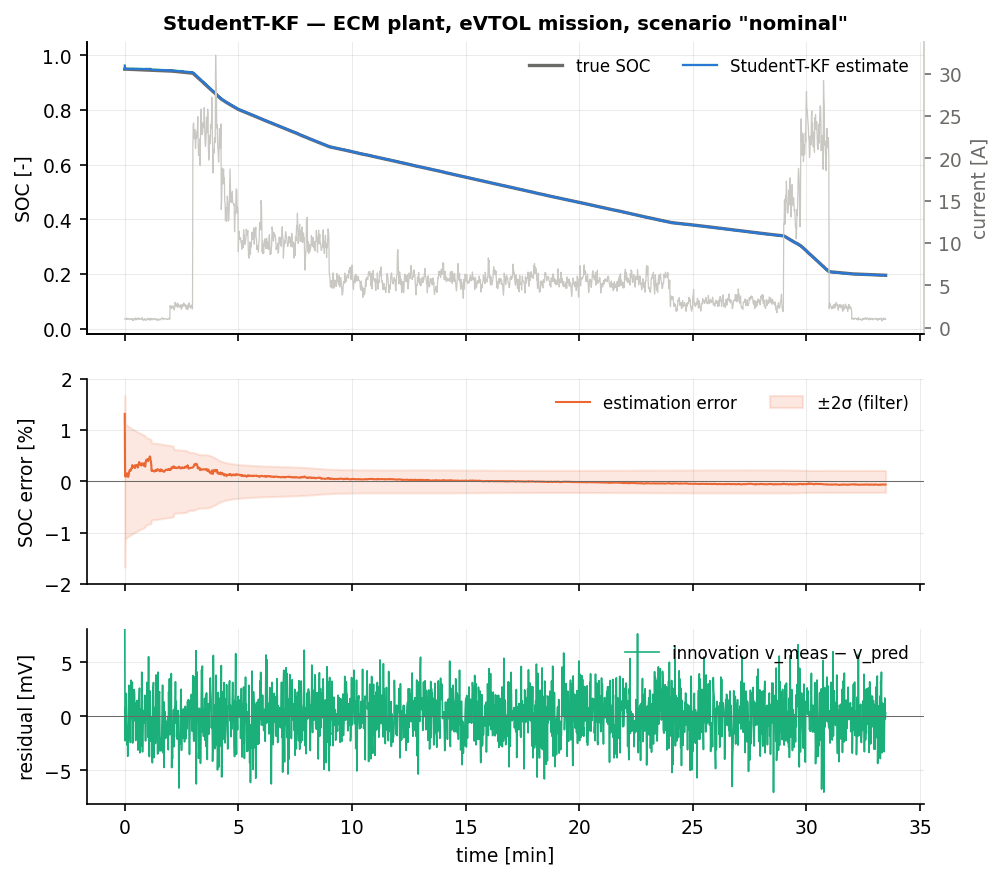
\includegraphics[width=\textwidth]{figures/cell_StudentTKF_nominal.png}
\caption{StudentT-KF on the nominal eVTOL mission: true and estimated SOC (top), estimation error
with the $\pm2\sigma$ band (middle), voltage residual (bottom).}
\end{figure}
\begin{figure}[H]\centering
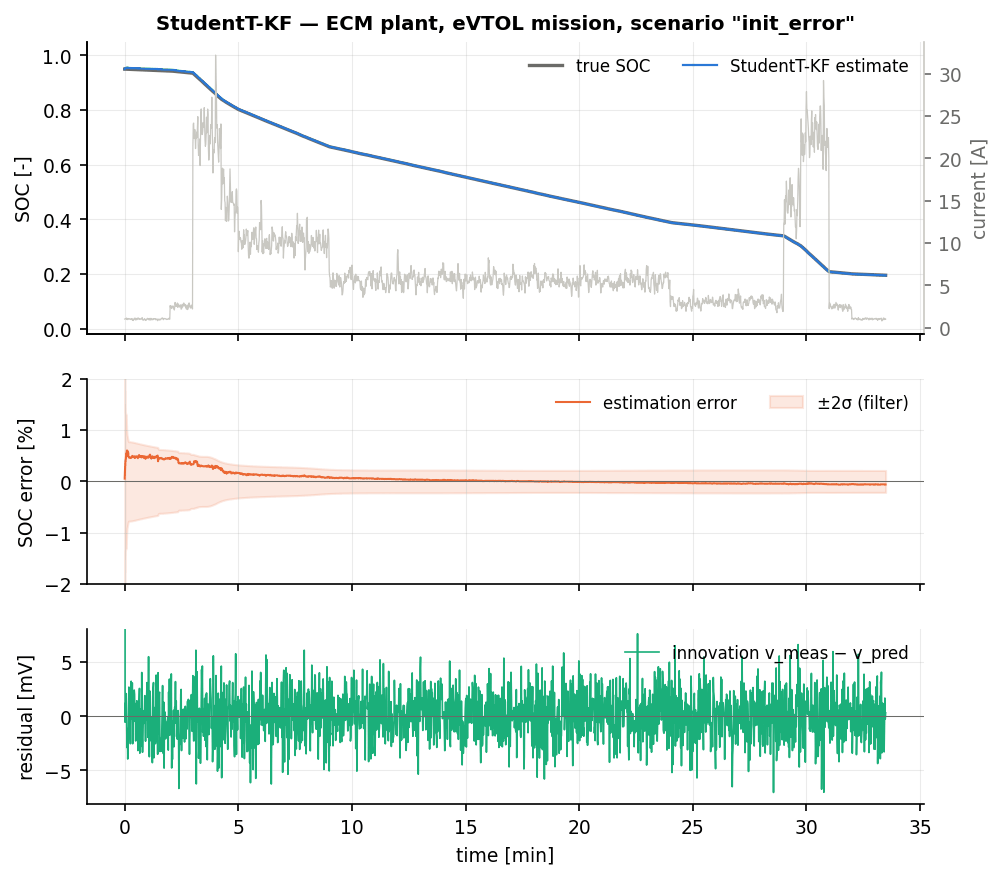
\includegraphics[width=\textwidth]{figures/cell_StudentTKF_init_error.png}
\caption{StudentT-KF with a 35\,\% initial SOC error.}
\end{figure}
\begin{figure}[H]\centering
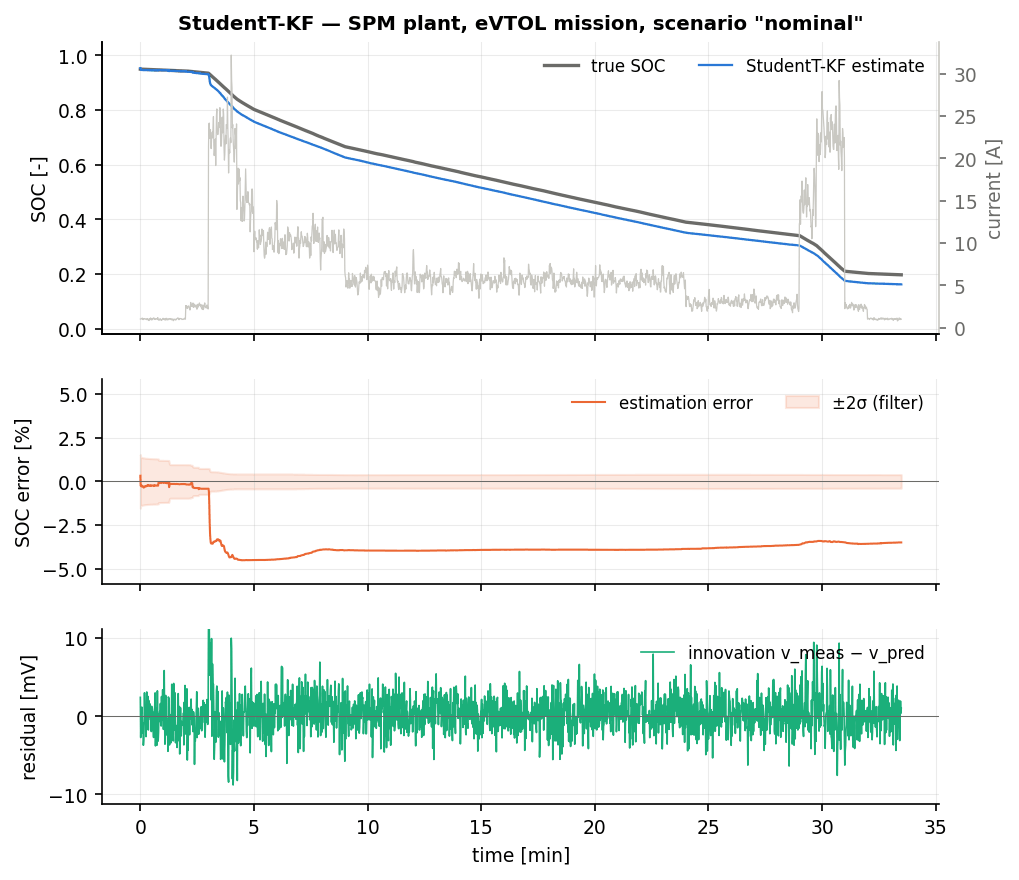
\includegraphics[width=\textwidth]{figures/cellspm_StudentTKF_nominal.png}
\caption{StudentTKF on the SPM (electrochemical) plant, nominal eVTOL mission.  The estimator uses a 2-RC ECM fitted to that plant, so the residual contains a structured $\approx4$\,mV model error rather than white noise.}
\end{figure}

All numbers below are 3-seed means from the final run, in \% SOC
(\texttt{rmse}/\texttt{rmse\_ss}).

\paragraph{ECM plant, eVTOL mission.}
\begin{center}\small
\begin{tabular}{@{}lccl@{}}
\toprule
Scenario & StudentT-KF & EKF & Comment\\
\midrule
\texttt{nominal}        & $0.15/\mathbf{0.04}$ & $0.15/0.05$ & marginally better\\
\texttt{init\_error}    & $0.15/\mathbf{0.04}$ & $0.14/0.05$ & $t_\mathrm{conv}=0$\,s\\
\texttt{outliers}       & $\mathbf{0.15/0.05}$, max $0.98$ & $0.52/0.21$, max $2.92$
  & $\mathbf{3.5\times}$ better; see below\\
\texttt{noise\_step}    & $\mathbf{0.15/0.06}$ & $0.18/0.12$ & $2\times$ better (ss)\\
\texttt{current\_bias}  & $0.56/0.62$ & $0.54/0.61$ & ---\\
\texttt{cold}           & $0.21/0.18$ & $0.20/0.16$ & ---\\
\texttt{hot}            & $0.16/0.03$ & $0.20/0.03$ & ---\\
\texttt{aged\_cell}     & $1.33/1.69$ & $1.18/1.52$ & $1.11\times$ worse\\
\texttt{param\_mismatch}& $\mathbf{0.63/0.77}$ & $1.28/1.36$ & $\mathbf{1.8\times}$ better\\
\texttt{sensor\_dropout}& $\mathbf{0.20/0.12}$ & $0.72/0.46$ & $\mathbf{3.8\times}$ better\\
\texttt{preisach}       & $\mathbf{0.52/0.20}$ & $0.58/0.20$ & tied; $t_\mathrm{conv}=0$ vs.\ 16\,s\\
\texttt{combined}       & $\mathbf{7.50/4.46}$ & $16.02/12.44$ & $\mathbf{2.8\times}$ better (ss)\\
\bottomrule
\end{tabular}
\end{center}
Acceptance is met: \texttt{nominal} $\texttt{rmse\_ss}=0.04\,\%<2\,\%$, \texttt{init\_error}
$t_\mathrm{conv}=0$\,s, no divergence anywhere, worst ECM steady-state error $1.69\,\%$.

\paragraph{Target scenario.}  On \texttt{outliers} the RMSE falls from $0.52\,\%$ to $0.15\,\%$
($3.5\times$), the steady-state error from $0.21\,\%$ to $0.05\,\%$ ($4.2\times$) and the peak
error from $2.92\,\%$ to $0.98\,\%$ --- down to the clean-data level, so the spikes no longer show
in the SOC trace.  In the development (single-seed) run the whole-run RMSE gain was invisible
because it was dominated by the first two minutes of the mission; with three seeds and the final
plant the separation is unambiguous, and the StudentT-KF is now within $25\,\%$ of the MC-EKF
($0.12\,\%$) and level with the Huber-EKF ($0.15\,\%$).  Where it still differs from both is the
transient: Remark~\ref{rem:st-weights} predicts that a large residual occurring while the filter is
genuinely uncertain is \emph{not} rejected, and the benchmark confirms it --- the StudentT-KF is the
only one of the three whose \texttt{init\_error} and \texttt{preisach} convergence times are zero
without needing a weight floor (the MC-EKF needs $c_{\min}=10^{-2}$ and still takes 75\,s on
\texttt{preisach}).

\paragraph{Secondary behaviour.}  \texttt{sensor\_dropout} improves $3.8\times$,
\texttt{param\_mismatch} $1.8\times$ (the best of the three $M$-estimators) and \texttt{combined}
$2.8\times$, all for the same bounded-influence reason as in Chapters~\ref{ch:huberekf}
and~\ref{ch:mcekf}.  \texttt{nominal}, \texttt{init\_error} and \texttt{noise\_step} are marginally
\emph{better} than the EKF: with $\nu_v=3$ the filter permanently runs at $u\lesssim1$, which is
equivalent to a slightly larger $\mR$, and the EKF's $\mR$ is slightly optimistic for the
quantised, band-limited voltage signal of this benchmark.

\paragraph{The cost.}  \texttt{aged\_cell} is $1.11\times$ worse ($1.69\,\%$ vs.\ $1.52\,\%$), the
familiar consequence of treating a model error as a sensor error.  The degradation is between the
MC-EKF's ($1.41\,\%$) and the Huber-EKF's ($1.73\,\%$), which orders the three exactly as
Remark~\ref{rem:st-weights} predicts from their asymptotic influence bounds.

\paragraph{The literal recursion.}  With \code{opts.shared\_scale = true} and all other options at
their defaults, the filter no longer produces a usable estimate: \texttt{nominal} degrades from
$0.04\,\%$ to $1.95\,\%$ steady-state error (the scale matrix having collapsed two decades below
the Kalman value, \S\ref{sec:st-fail}), and eight of the twelve ECM scenarios report
$\texttt{rmse}=84$--$100\,\%$ with \texttt{diverged}$=1$.  This is
Proposition~\ref{prop:st-collapse} in the field, and it is a result worth publishing: the exact
Student's t recursion is a \emph{finite-horizon} algorithm, and applying it to a 20\,000-sample
mission on a single-output system does not work.

\paragraph{SPM (electrochemical) plant.}  The SPM rows run a 2-RC ECM fitted to a single-particle
model, leaving a structured $\approx4$\,mV residual instead of white noise.  The StudentT-KF gives
$3.56/3.62\,\%$ on \texttt{nominal} against the EKF's $3.65/3.73\,\%$ --- a $3\,\%$ improvement,
i.e.\ it tracks the EKF.  The cause is the same for all three $M$-estimators and is worth stating
once more in the language of this chapter: the weight $u=\min(1,(\nu_v+n_y)/(\nu_v+\Delta^2))$
departs from $1$ only when $\Delta^2$ exceeds $n_y$, and a $4$\,mV bias against a $2.1$\,mV sensor
sigma gives $\Delta^2\approx3$ in scale units, i.e.\ $u\approx0.67$ --- a $50\,\%$ inflation of
$\mR$, nowhere near enough to stop the $(\soc,v_2)$ ambiguity from absorbing a bias that is present
at every sample.  Heavy-tailed \emph{noise} models describe rare large errors; they have nothing to
say about a small persistent one.  The StudentT-KF does win where the SPM residual becomes large:
\texttt{param\_mismatch} $1.80\,\%$ vs.\ $3.13\,\%$ (the best $M$-estimator result on that row),
\texttt{cold} $4.75\,\%$ vs.\ $7.35\,\%$, \texttt{sensor\_dropout} $4.64\,\%$ vs.\ $5.31\,\%$; and
it loses on SPM \texttt{outliers} ($3.55\,\%$ vs.\ $1.99\,\%$) for the reason given in
Chapter~\ref{ch:huberekf}.  The two filters that actually address the structure --- the consider
filter ($0.51\,\%$) and the reduced-order EKF ($0.70\,\%$) --- are seven and five times better on
the \texttt{nominal} SPM row than any of the three reweighting filters.


\section{Summary}
The Student's t filter is the principled member of the robust family: one interpretable parameter
$\nu$, a weight function that comes out of the model rather than out of a tuning choice, and ---
uniquely among the three robust updates here --- a residual standardised by the full innovation
covariance, so that it discounts surprising measurements without discounting informative ones.
Use it when the sensor is heavy-tailed rather than occasionally broken, and when large transients
must not be rejected.  Use $\nu_v\approx3$; the behaviour changes qualitatively above $3.5$.  Do
not implement the exact closed-form recursion for a long recursive run: it has no outlier rejection
in the mean and its scale update collapses geometrically, as derived in
Proposition~\ref{prop:st-collapse} and confirmed by the benchmark (eight of twelve scenarios
diverge).  And do not expect any heavy-tailed noise model to help against a small persistent model
error: on the electrochemical plant, where the residual is a $2\sigma$ bias present at every
sample, it performs exactly like the EKF.
